% \documentclass[a4paper, conference, compsoc]{IEEEtran}
\documentclass[12pt,a4paper]{article}
% \documentclass[%
%     pdftex,
%     oneside,			% Einseitiger Druck.
%     12pt,				% Schriftgroesse
%     parskip=half,		% Halbe Zeile Abstand zwischen Absätzen.
% %	topmargin = 10pt,	% Abstand Seitenrand (Std:1in) zu Kopfzeile [laut log: unused]
%     headheight = 12pt,	% Höhe der Kopfzeile
% %	headsep = 30pt,	% Abstand zwischen Kopfzeile und Text Body  [laut log: unused]
%     headsepline,		% Linie nach Kopfzeile.
%     footsepline,		% Linie vor Fusszeile.
%     footheight = 16pt,	% Höhe der Fusszeile
%     abstracton,		% Abstract Überschriften
%     DIV=calc,		% Satzspiegel berechnen
%     BCOR=8mm,		% Bindekorrektur links: 8mm
%     headinclude=false,	% Kopfzeile nicht in den Satzspiegel einbeziehen
%     footinclude=false,	% Fußzeile nicht in den Satzspiegel einbeziehen
%     listof=totoc,		% Abbildungs-/ Tabellenverzeichnis im Inhaltsverzeichnis darstellen
%     toc=bibliography,	% Literaturverzeichnis im Inhaltsverzeichnis darstellen
% ]{scrreprt}	% Koma-Script report-Klasse, fuer laengere Bachelorarbeiten alternativ auch: scrbook


% Basic packages
\usepackage[T1]{fontenc}
\usepackage[utf8]{inputenc}
\usepackage[scaled]{beramono}
\usepackage[english,ngerman]{babel,varioref}
\usepackage{xcolor}
\usepackage{amsmath}

% Tables
\usepackage{booktabs}
\usepackage{multirow}
\usepackage{longtable}
% Graphics and Includes
\usepackage[pdftex]{graphicx}
\graphicspath{{assets/img/}}
\DeclareGraphicsExtensions{.pdf,.jpeg,.png,.jpg}
\usepackage{tikz}
\usetikzlibrary{arrows.meta,bending,automata,shapes}
\usepackage[underline=true,rounded corners=false]{pgf-umlsd}

% Reduce distance before caption
\usepackage[skip=5pt]{caption}
% Bibliography
\usepackage[backend=biber, isbn=false, doi=false, style=ieee]{biblatex}
\addbibresource{bibliography.bib}
\AtBeginBibliography{\raggedright}
%\nocite{*}

% Gossar z.a. für acronyme
% \usepackage[acronym]{glossaries}
% \makeglossaries
\usepackage[printonlyused]{acronym} % falls gewünscht kann die Option footnote eingefügt werden, dann wird die Erklärung nicht inline sondern in einer Fußnote dargestellt

% \section*{Abkürzungsverzeichnis}
\begin{acronym}[AAAAAAA]
    \acro{fe}[F\&E]{Forschung und Entwicklung}
    \acro{parc}[PARC]{Palo Alto Research Center}
    \acro{sac}[SAC]{SAP Analytics Cloud}
\end{acronym}

% Colors
\definecolor{ListingBackground}{HTML}{E6E6E6}
\definecolor{LinkColor}{HTML}{000000}


% Font
\usepackage[onehalfspacing]{setspace}
\usepackage{lmodern}
\usepackage[official]{eurosym}
\usepackage{enumitem}
\usepackage[locale=DE]{siunitx} % SI Units für Währungen
\DeclareSIUnit{\EUR}{\text{\euro}} % Beispielverwendung: \SI{10.10}{\EUR}

\usepackage[autostyle=true,german=quotes]{csquotes}
\usepackage{url}
\newcommand{\code}[1]{\texttt{#1}}

% Additional Setup
\usepackage[unicode=true,hypertexnames=false,colorlinks=true,linkcolor=LinkColor,citecolor=LinkColor,urlcolor=LinkColor,pdftex]{hyperref}

% Trennung von URLs im Literaturverzeichnis (große Werte [> 10000] verhindern die Trennung)
\defcounter{biburlnumpenalty}{10} % Strafe für Trennung in URL nach Zahl
\defcounter{biburlucpenalty}{500}  % Strafe für Trennung in URL nach Großbuchstaben
\defcounter{biburllcpenalty}{500}  % Strafe für Trennung in URL nach Kleinbuchstaben
\interfootnotelinepenalty=10000 % prevent all footnotes from breaking over a page.

% Configs
\setcounter{tocdepth}{1} % Limit table of contents to subsection
\sisetup{detect-weight=true, detect-family=true} % SI Units shall detect font weight and family
\setlist[description]{style=nextline} % Break definitions of terms to a new line (used by \begin{description} \item[foo] bar \end{description})
\renewcommand*{\bibfont}{\small}

%Hurenkinder und Schusterjungen vermeiden
\clubpenalty = 10000
\widowpenalty = 10000
\displaywidowpenalty = 10000

% Quellcode
\usepackage{listings}
\usepackage{float}
\usepackage{textcomp}
\lstset{
    inputpath=assets/listings,
    language=Java,			% Standardsprache des Quellcodes
    numbers=left,			% Zeilennummern links
    stepnumber=1,			% Jede Zeile nummerieren.
    numbersep=5pt,			% 5pt Abstand zum Quellcode
    numberstyle=\tiny,		% Zeichengrösse 'tiny' für die Nummern.
    breaklines=true,		% Zeilen umbrechen wenn notwendig.
    breakautoindent=true,	% Nach dem Zeilenumbruch Zeile einrücken.
    postbreak=\space,		% Bei Leerzeichen umbrechen.
    tabsize=2,				% Tabulatorgrösse 2
    basicstyle=\ttfamily\footnotesize, % Nichtproportionale Schrift, klein für den Quellcode
    showspaces=false,		% Leerzeichen nicht anzeigen.
    showstringspaces=false,	% Leerzeichen auch in Strings ('') nicht anzeigen.
    extendedchars=true,		% Alle Zeichen vom Latin1 Zeichensatz anzeigen.
    captionpos=b,			% sets the caption-position to bottom
    backgroundcolor=\color{ListingBackground}, % Hintergrundfarbe des Quellcodes setzen.
    xleftmargin=0pt,		% Rand links
    xrightmargin=0pt,		% Rand rechts
    frame=single,			% Rahmen an
    frameround=ffff,
    rulecolor=\color{darkgray},	% Rahmenfarbe
    fillcolor=\color{ListingBackground},
    keywordstyle=\color[rgb]{0.133,0.133,0.6},
    commentstyle=\color[rgb]{0.133,0.545,0.133},
    stringstyle=\color[rgb]{0.627,0.126,0.941},
    float,
    upquote=true
}


\colorlet{punct}{red!60!black}
\definecolor{delim}{RGB}{20,105,176}
\colorlet{numb}{magenta!60!black}

\lstdefinelanguage{json}{
    string=[s]{"}{"},
    stringstyle=\color{numb},
    literate=
     *{0}{{{\color{numb}0}}}{1}
      {1}{{{\color{numb}1}}}{1}
      {2}{{{\color{numb}2}}}{1}
      {3}{{{\color{numb}3}}}{1}
      {4}{{{\color{numb}4}}}{1}
      {5}{{{\color{numb}5}}}{1}
      {6}{{{\color{numb}6}}}{1}
      {7}{{{\color{numb}7}}}{1}
      {8}{{{\color{numb}8}}}{1}
      {9}{{{\color{numb}9}}}{1}
      {:}{{{\color{punct}{:}}}}{1}
      {,}{{{\color{punct}{,}}}}{1}
      {\{}{{{\color{delim}{\{}}}}{1}
      {\}}{{{\color{delim}{\}}}}}{1}
      {[}{{{\color{delim}{[}}}}{1}
      {]}{{{\color{delim}{]}}}}{1}
}

\lstdefinelanguage{yaml}{
  identifierstyle=\color{delim},
  sensitive=false,
  comment=[l]{\#},
  commentstyle=\color{purple}\ttfamily,
  stringstyle=\color{numb},
  morestring=[b]',
  morestring=[b]"
}

\lstloadlanguages{Python,Java,bash}
% Useful tools
\usepackage{blindtext}
\usepackage{lipsum}
\usepackage[section]{placeins} % Prevent figures and tables to float to new section
\usepackage[obeyFinal,backgroundcolor=yellow,linecolor=black]{todonotes}


%Angaben zur Arbeit
\def\myTitel{Ein ansprechender Titel}
\def\myArbeit{Seminararbeit}
\def\myFach{Spanndendes Fach}
\def\myDatum{\today}
\def\myBetreuer{Netter Betreuer}
\def\myGutachter{Strenger Gutachter}
\def\myBearbeitungszeit{Lange}
\def\myAbgabeort{Heilbronn}

%Angaben zur Person
\def\myAutor{Wunderbarer Autor}
\def\myDegree{Master Informatik}
\def\myInstitution{DHBW CAS, Bildungscampus 13, 74076 Heilbronn}
\def\myMatrikelnr{123456}
\def\myKurs{TMINF17}
\def\myFirma{SAP SE}
\def\myFirmenort{Walldorf}
%\section*{Abkürzungsverzeichnis}
\begin{acronym}[AAAAAAA]
    \acro{fe}[F\&E]{Forschung und Entwicklung}
    \acro{parc}[PARC]{Palo Alto Research Center}
    \acro{sac}[SAC]{SAP Analytics Cloud}
\end{acronym}

\begin{document}


\title{\myTitel}
\author{\myAutor~(\myMatrikelnr)\\
    \small{\myFach}\\
    \small{\myDegree}\\
    \small{\myInstitution}
}
\date{\myDatum}

\begin{titlepage}
	\begin{longtable}{p{8.2cm} p{5.4cm}}
		% Firmenlogo
		&
		
\includegraphics[width=5.4cm]{casLogo}
	\end{longtable}
	\addtocounter{table}{-1}
    {\let\newpage\relax\maketitle}
    \thispagestyle{empty}
    % \vfill
    \begin{abstract}
    \textit{Open} und \textit{Closed Innovation} sind zwei Herangehensweisen
    um den Wissensaustausch zwischen einem Unternehmen
     und dessen Umwelt im Rahmen der Entwicklung von Innovationen zu organisieren.
    Diese Seminararbeit widmet sich der \textit{Closed Innovation}.
    Hierzu wird diese vorgestellt und einer Bewertung unterzogen.
    Die Anwendung der Methode wird anhand der Firmen \textit{Xerox} und \textit{IBM} beschrieben.
    Zusätzlich wird diesbezüglich der Innovationsprozess bei \textit{SAP} betrachtet.
\end{abstract}
\end{titlepage}
% \begin{titlepage}
	\begin{longtable}{p{8.2cm} p{5.4cm}}
		% Firmenlogo
		&
		
\includegraphics[width=5.4cm]{casLogo}
	\end{longtable}
	\addtocounter{table}{-1}
	\enlargethispage{20mm}
	\begin{center}
		\vspace*{12mm}	{\LARGE\textbf \myTitel }\\
		\vspace*{12mm}	{\large\textbf \myArbeit}\\
		% \vspace*{12mm}	\langdeckblattabschlusshinleitung\\
		\vspace*{3mm}		{\textbf \myDegree}\\
		\vspace*{12mm}	des Studiengangs \myKurs\\
    \vspace*{3mm}		am DHBW CAS\\
		\vspace*{12mm}	von\\
		\vspace*{3mm}		{\large\textbf \myAutor}\\
		\vspace*{12mm}	\myDatum\\
	\end{center}
	\vfill
	\begin{spacing}{1.2}
	\begin{tabbing}
		mmmmmmmmmmmmmmmmmmmmmmmmmm             \= \kill
		\textbf{Bearbeitungszeit}       \>  \myBearbeitungszeit\\
		\textbf{Matrikelnummer, Kurs}  \>  \myMatrikelnr, \myKurs\\
		\textbf{Firma}                  \>  \myFirma, \myFirmenort\\
		\textbf{Betreuer}               \>  \myBetreuer\\
		\textbf{Gutachter}              \>  \myGutachter
	\end{tabbing}
	\end{spacing}
\end{titlepage}

\pagenumbering{Roman}

% Sperrvermerk
% \thispagestyle{empty}
% Sperrvermerk direkt hinter Titelseite
\section*{Sperrvermerk}

\vspace*{2em}

Die vorliegende {\myArbeit} mit dem Titel {\itshape{} \myTitel{}\/}
enthält unternehmensinterne bzw. vertrauliche Informationen der {\myFirma},
ist deshalb mit einem Sperrvermerk versehen
und wird ausschließlich zu Prüfungszwecken am Studiengang
{\myDegree} der Dualen Hochschule Baden-Württemberg vorgelegt.
Sie ist ausschließlich zur Einsicht durch den zugeteilten Gutachter,
die Leitung des Studiengangs und ggf. den Prüfungsausschuss des Studiengangs
bestimmt.  Es ist untersagt,
\begin{itemize}
\item den Inhalt dieser Arbeit (einschließlich Daten, Abbildungen, Tabellen, Zeichnungen usw.) als Ganzes oder auszugsweise weiterzugeben,
\item Kopien oder Abschriften dieser Arbeit (einschließlich Daten, Abbildungen, Tabellen, Zeichnungen usw.) als Ganzes oder in Auszügen anzufertigen,
\item diese Arbeit zu veröffentlichen bzw. digital, elektronisch oder virtuell zur Verfügung zu stellen.
\end{itemize}
Jede anderweitige Einsichtnahme und Veröffentlichung – auch von Teilen der Arbeit – bedarf der vorherigen Zustimmung durch den Verfasser und {\myFirma}.

\vspace{3em}

\myAbgabeort, \myDatum
\vspace{4em}

\rule{6cm}{0.4pt}\\
\myAutor

% \newpage

% Erklärung
\thispagestyle{empty}

\section*{Selbstständigkeitserklärung}
\vspace*{2em}


Ich versichere hiermit, dass ich meine {\myArbeit} mit dem Thema: {\itshape \myTitel } selbstständig verfasst und keine anderen als die angegebenen Quellen und Hilfsmittel benutzt habe. Ich versichere zudem, dass die eingereichte elektronische Fassung mit der gedruckten Fassung übereinstimmt.


\vspace{3em}

\myAbgabeort, \myDatum
\vspace{4em}

\rule{6cm}{0.4pt}\\
\myAutor

\newpage


% \begin{abstract}
    \textit{Open} und \textit{Closed Innovation} sind zwei Herangehensweisen
    um den Wissensaustausch zwischen einem Unternehmen
     und dessen Umwelt im Rahmen der Entwicklung von Innovationen zu organisieren.
    Diese Seminararbeit widmet sich der \textit{Closed Innovation}.
    Hierzu wird diese vorgestellt und einer Bewertung unterzogen.
    Die Anwendung der Methode wird anhand der Firmen \textit{Xerox} und \textit{IBM} beschrieben.
    Zusätzlich wird diesbezüglich der Innovationsprozess bei \textit{SAP} betrachtet.
\end{abstract}
% \newpage

\pagestyle{plain}		% nur Seitenzahlen im Fuß

% Inhaltsverzeichnis
\begin{spacing}{1.1}
    \begingroup
        \pagestyle{empty}
        %für die Anzeige von Unterkapiteln im Inhaltsverzeichnis
        \setcounter{tocdepth}{2}

        \tableofcontents
        \clearpage
    \endgroup
\end{spacing}
\newpage

% Abkürzungsverzeichnis
\cleardoublepage
\section*{Abkürzungsverzeichnis}
\begin{acronym}[AAAAAAA]
    \acro{fe}[F\&E]{Forschung und Entwicklung}
    \acro{parc}[PARC]{Palo Alto Research Center}
    \acro{sac}[SAC]{SAP Analytics Cloud}
\end{acronym}


% Abbildungsverzeichnis
\listoffigures

%Tabellenverzeichnis
% \cleardoublepage
% \listoftables

% % Quellcodeverzeichnis
% \cleardoublepage
% \lstlistoflistings

\cleardoublepage

\pagenumbering{arabic}

\section{Einleitung}\label{sec:einleitung}

Innovationen sind einer der wichtigsten Aspekte für ein Unternehmen um erfolgreich zu sein und zu bleiben.
Von Beginn an ist das Gebiete der Informationstechnologie von solchen Innovationen getrieben.

Vom ersten Computer über Smartphones bis hin zu Themen wie künstlicher Intelligenz,
all dies begann als eine Idee und wurde schließlich zur Innovation.

In der Praxis finden sich viele verschiedene Arten,
wie sich für ein Unternehmen ein sogenannter \textit{Innovationsprozess} etablieren lässt.

Mit \textit{Open} und \textit{Closed Innovation} führt Henry W. Chesbrough
in \cite{chesbrough2003} erstmals die Begriffe \textit{Open} und
\textit{Closed Innovation} ein.
Mit diesen Begriffen bennent er zwei Paradigmen, welche den Innovationsprozess im Hinblick auf die
Interaktion mit der Umwelt des Unternehmens und dem Fluss von Wissen betrachtet.

Die \textit{Closed Innovation}, mit welcher sich diese Seminararbeit haupsächlich befasst,
fokusiert sich hierbei auf das eigene Unternehmen, während sich die \textit{Open Innovation}
nach Außen hin öffnet.

In den folgenden Kapitel wird die \textit{Open Innovation} sowie grundlegend deren Gegenstück betrachtet.
Doch zunächst folgt die Erläuterung der Grundbegriffe \textit{Innovaiton} und \textit{Innovationsprozess}.
\section{Grundlagen}\label{sec:grundlagen}
\textit{Closed Innovation} ist eine Variante den Wissensaustausch
zur Entwicklung einer \textit{Innovation}
innerhalb eines \textit{Innovationsprozesses} zu organisieren.

In der Litaratur finden sich für die beiden letzeren Begriffe verschiedene Beschreibungen.
Im folgenden werden die in dieser Arbeit verwendeten Definitionen vorgestellt.

\subsection{Innovation}\label{sec:grundlagen-inno}
Bevor die Begriffe \textit{Closed} und \textit{Open Innovation} näher betrachtet werden,
ist es notwendig den Begriff \textit{Innovation} an sich zu definieren.
Verschiedene Autoren definieren diesen Begriff auf unterschiedliche Arten.
In \cite[5]{hauschildt2016innovationsmanagement} ist eine Auswahl verschiedener Definitionen dargestellt.
Diese werden zusammengefasst zu der allgemeinen Aussage:
\begin{quote}
    \enquote{Innovationen sind qualitativ neuartige Produkte oder Verfahren,
    die sich gegenüber einem Vergleichszustand \enquote{merklich} [...] unterscheiden}
    \cite[4]{hauschildt2016innovationsmanagement}
\end{quote}

In \cite[9]{herzog2011} wird ein solches neuartiges Produkt oder Verfahen als \textit{Invention} bezeichnet und erst durch kommerzielle Verwertung zur \textit{Innovation}.
Die vorliegende Arbeit folgt dieser Definition.
Es gilt somit:
\begin{equation*}
    Innovation = Invention + kommerzielle~Verwertung
\end{equation*}

Hierbei ist zu beachten, dass der Begriff sich nicht nur auf Produkte bezieht, welche vermarktet werden,
sonder auch auf Prozesse, welche innerhalb der Produktion genutzt werden.

\subsection{Innovationsprozess}\label{sec:grundlagen-prozess}
Um Ideen und Innovationen zu entwickeln und zu vermarkten durchlaufen diese zunächst einen Innovationsprozess.
Nach \cite[10\psq]{herzog2011} besteht dieser Prozess aus drei Phasen:
\begin{enumerate}
    \item Im \textit{Frontend of Innovation} werden neue Ideen geschaffen, ausgewählt, sowie auf technologische Machbarkeit und mögliche Marktakzeptanz hin bewertet.
    \item Anschließend werden ausgewählte Ideen realisiert und entwickelt.
    \item Zuletzt wird die Vermarktung der Entwicklungsergebnisse geplant und durchgeführt.
\end{enumerate}

\subsection{Closed Innovation}\label{sec:grundlagen-closed}

\paragraph{Ursprung}
Das \textit{Closed Innovation}-Modell ist das vorherschende Innovationsmodell im 20. Jahrhundert.
Es spiegelt die damals vorherschende Wissensumgebung wider.
Unter Wissenschaftlern ist es verpönt ihre Fähigkeiten zu Nutzen um wirtschaftliche Probleme zu lösen.

Um dennoch Innovationen anzutreiben und so den kommerziellen Erfolg zu sichern,
sind Unternhemen gezwungen selbst in \ac{fe} zu investieren.
Da in anderen Unternehmen das notwendige Wissen nicht aufgebaut ist,
müssen Unternehmen innerhalb ihrer \ac{fe}-Organisation das gesamte Spektrum von den Grundlagen bis hin zum fertigen Produkt abdecken.
Voraussetzung hierfür ist die Akquise von talentierten Mitarbeitern.

\todo[inline]{Geschichte etwas ausführlicher}

\paragraph{Prinzipien}
Implizit ergeben sich so die Prinzipien der \textit{Closed Innovation} (nach \cite[19]{herzog2011}):
\begin{itemize}
    \item Ein Unternehmen sollte die talentiertesten Mitarbeiter anstellen.
    \item Um von Innovationen zu profitieren, müssen diese innerhalb des Unternehmens den gesamten Innovationsprozess durchlaufen (Vom Entdecken, über das Entwicklen bis hin zur Vermarktung)
    \item Um ein Produkt als erstes auf den Markt zu bringen, muss eine Entdeckung innerhalb des eingenen Unternehmens entstehen.
    \item Durch die Markteinführung als erstes Unternehmen gewinnt es den Wettbewerb
    \item Investiert ein Unternehmen am meisten in \ac{fe}, so entstehen dort die besten Ideen, was wiederum den Wettbewerb gewinnt.
    \item Damit andere Unternehmen nicht von den eigenen Entdeckungen profitieren, gilt es das geistige Eigentum zu schützen.
\end{itemize}

\paragraph{Modell}
Aus diesen Regeln folgt das in \autoref{fig:closedInnovation} dargestellte Modell.
Der gesamte Innovatoinsprozess spielt sich innerhalb der Grenzen des Unternehmes ab.
Eine Innovation beginnt immer durch eine Idee innerhalb des Unternehmens,
wird durch die firmeneigene \ac{fe}-Abteilung entwickelt
und schließlich auf dem bestehenden Markt des Unternehmens kommerzialisiert.

\begin{figure}[ht!]
    \centering
    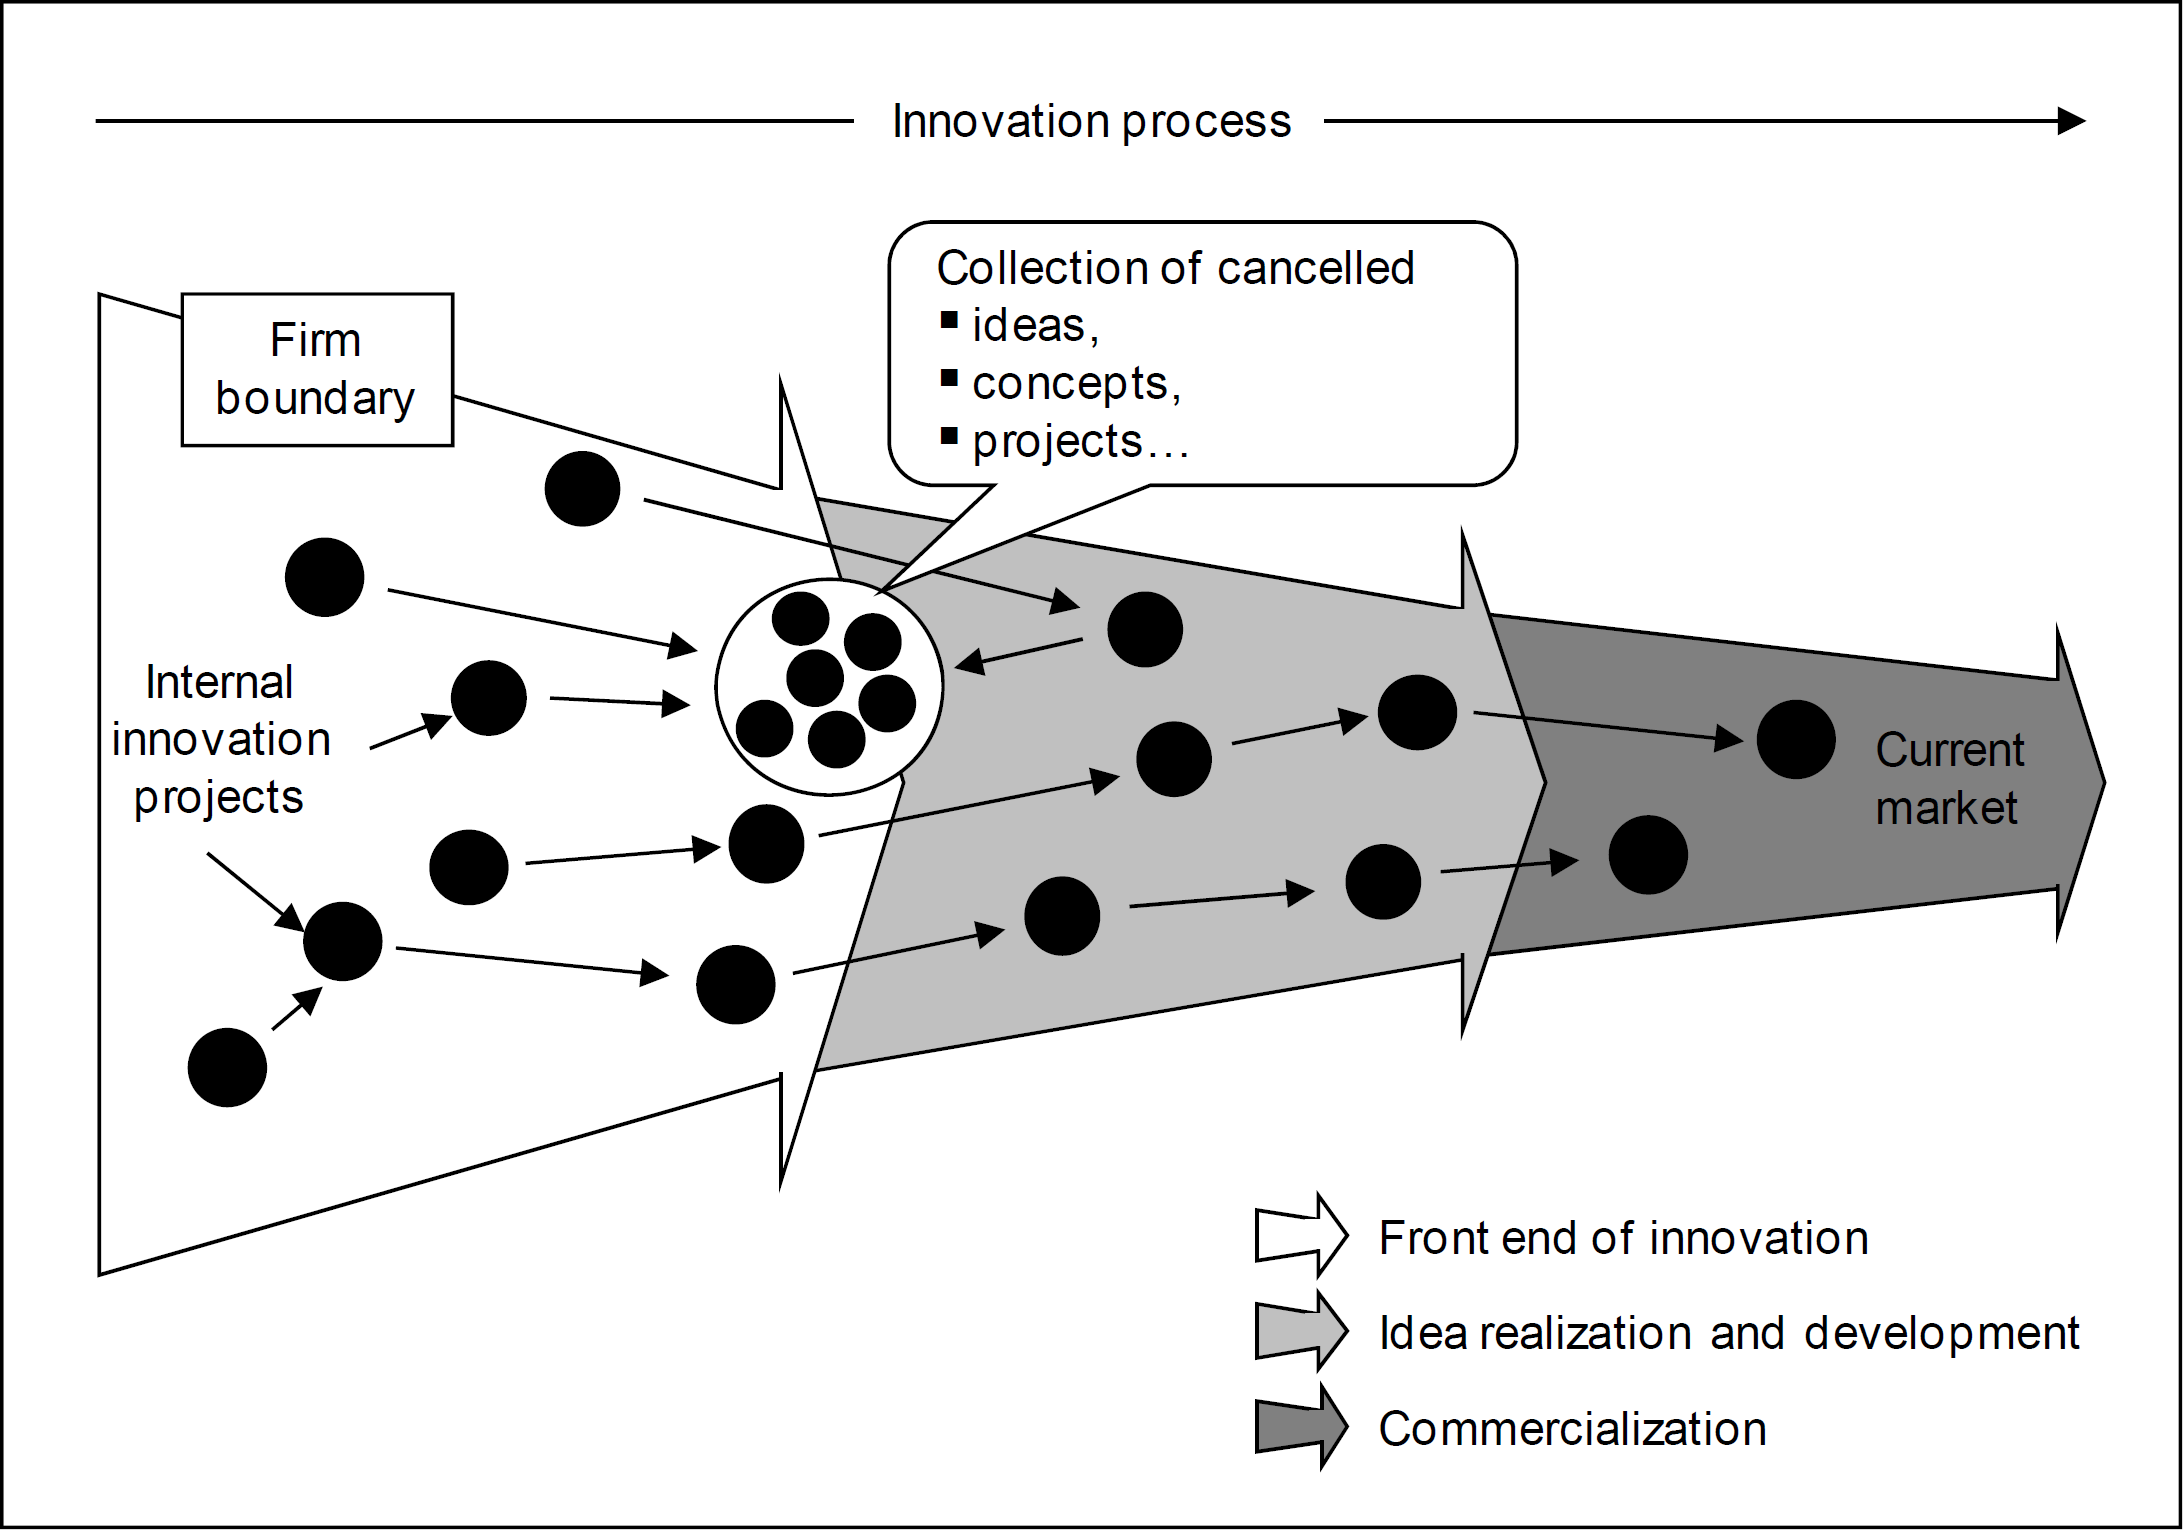
\includegraphics[width=1\textwidth]{ClosedInnovation}
    \caption{Closed Innovation Modell (aus \cite[20]{herzog2011})}
    \label{fig:closedInnovation}
\end{figure}

Selbstverständlich können nicht alle Ideen realisiert werden.
Möglicherweise ist die Ursache hierfür fehlende Ressourcen (Arbeitskraft oder Wissen)
oder es findet sich innerhalb der Unternehmensgrenzen keine vermarktbare Anwendung für eine neue Entdeckung.
Auch werden Ideen gegebenenfalls nicht umgesetzt, da vermutet wird, dass keine Akzeptanz am Markt herrscht.

Abgelehnte Ideen und abgebrochene Projekte werden beispielsweise in Datenbanken gesammelt.
Von dort werden sie wieder aufgegriffen oder bleiben ein ungenutzer Teil des geistigen Eigentums einer Unternehmens.


\subsection{Open Innovation}\label{sec:grundlagen-open}

Das Modell der \textit{Open Innovation} ist -- schon rein namentlich -- der Gegensatz der \textit{Closed Innovation}.
Da der Fokus dieser Arbeit auf letzerem liegt,
wird im Folgenden der offene Ansatz lediglich oberflächlich behandelt.
\todo[inline]{... um später besser Vergliechen zu können?}

\begin{figure}[ht!]
    \centering
    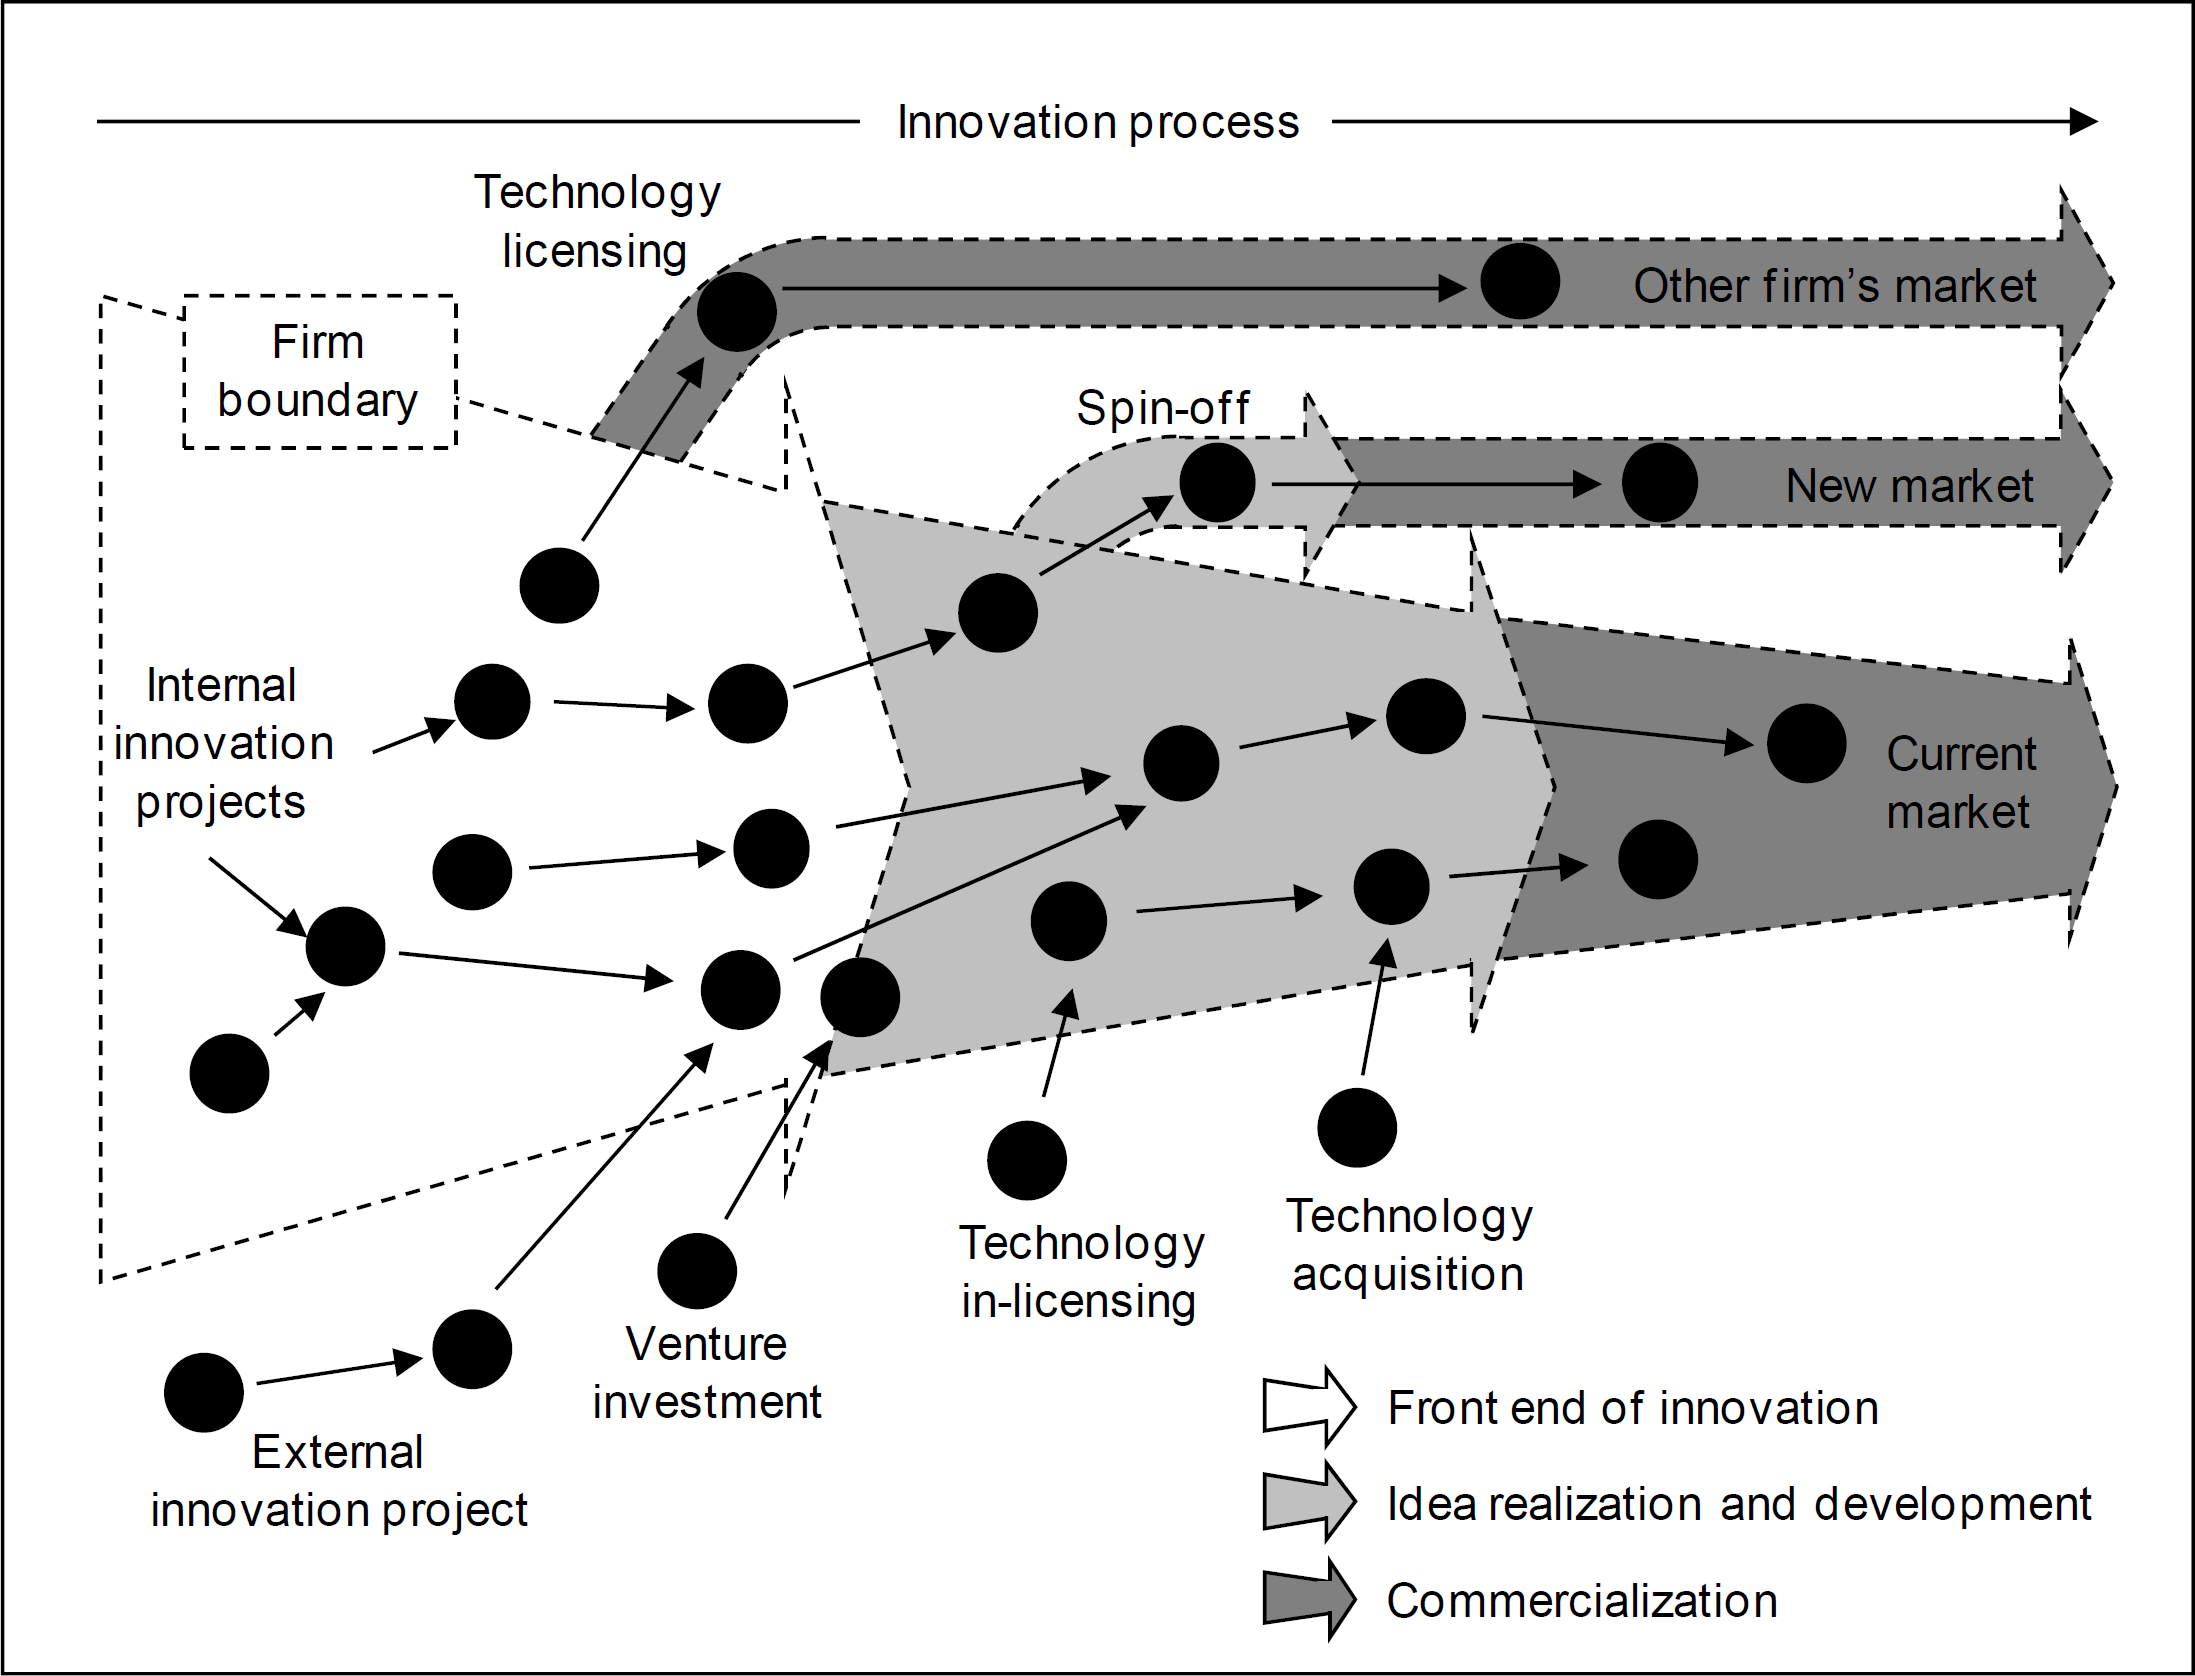
\includegraphics[width=1\textwidth]{OpenInnovation}
    \caption{Open Innovation Modell (aus \cite[23]{herzog2011})}
    \label{fig:openInnovation}
\end{figure}

Wie in \autoref{fig:openInnovation} zu sehen,
sind in der \textit{Open Innovation} die Grenzen eines Unternehmens \enquote{löchrig}.
Dies bedeutet, dass zusätzlich zu den intern entstandenen und entwickelten Innovationen
zusätzlich jederzeit Wissen von außen in den Innovationsprozess einfließt
und Projekte, welche innerhalb des Unternehmens nicht weiter verfolgt werden,
veröffentlicht werden oder genutz werden um neue Märkte zu erschließen.

Details zum \textit{Closed Innovation}-Ansatz können in unter Anderem
in \cite[60\psqq]{chesbrough2003} und \cite[21\psqq]{herzog2011} nachgelesen werden.
\newpage
\section{Closed Innovation}\label{sec:grundlagen-closed}

\subsection{Ursprung}
Das \textit{Closed Innovation}-Modell ist das vorherrschende Innovationsmodell im 20. Jahrhundert.
Es spiegelt die damalige Wissensumgebung wider.
Unter Wissenschaftlern ist es verpönt ihre Fähigkeiten zu nutzen, um wirtschaftliche Probleme zu lösen.

Um dennoch Innovationen anzutreiben und so den kommerziellen Erfolg zu sichern,
sind Unternehmen gezwungen selbst in \ac{fe} zu investieren.
Da auch bei Zulieferern das notwendige Wissen nicht aufgebaut ist,
müssen Unternehmen innerhalb ihrer \ac{fe}-Organisation das gesamte Spektrum von den Grundlagen bis hin zum fertigen Produkt abdecken.
Voraussetzung hierfür ist die Akquise von talentierten Mitarbeitern.

\subsection{Prinzipien}
Implizit ergeben sich so die Prinzipien der \textit{Closed Innovation} (nach \cite[19]{herzog2011}):
\begin{itemize}
    \item Ein Unternehmen sollte die talentiertesten Mitarbeiter anstellen.
    \item Um von Innovationen zu profitieren, müssen diese innerhalb des Unternehmens den gesamten Innovationsprozess durchlaufen (Vom Entdecken, über das Entwickeln bis hin zur Vermarktung).
    \item Um ein Produkt als erstes auf den Markt zu bringen, muss eine Entdeckung innerhalb des eigenen Unternehmens entstehen.
    \item Bringt ein Unternehmen ein Produkt zuerst auf den Markt, so gewinnt es den Wettbewerb.
    \item Investiert ein Unternehmen am meisten in \ac{fe}, so entstehen dort die besten Ideen, was wiederum den Wettbewerb gewinnen lässt.
    \item Damit andere Unternehmen nicht von den eigenen Entdeckungen profitieren, gilt es das geistige Eigentum zu schützen.
\end{itemize}

\subsection{Modell}
Aus diesen Regeln folgt das in \autoref{fig:closedInnovation} dargestellte Modell.
Der gesamte Innovationsprozess spielt sich innerhalb der Grenzen des Unternehmens ab.
Eine Innovation beginnt immer mit einer Idee innerhalb des Unternehmens,
wird durch die firmeneigene \ac{fe}-Abteilung entwickelt
und schließlich auf dem bestehenden Markt des Unternehmens kommerzialisiert.

\begin{figure}[ht!]
    \centering
    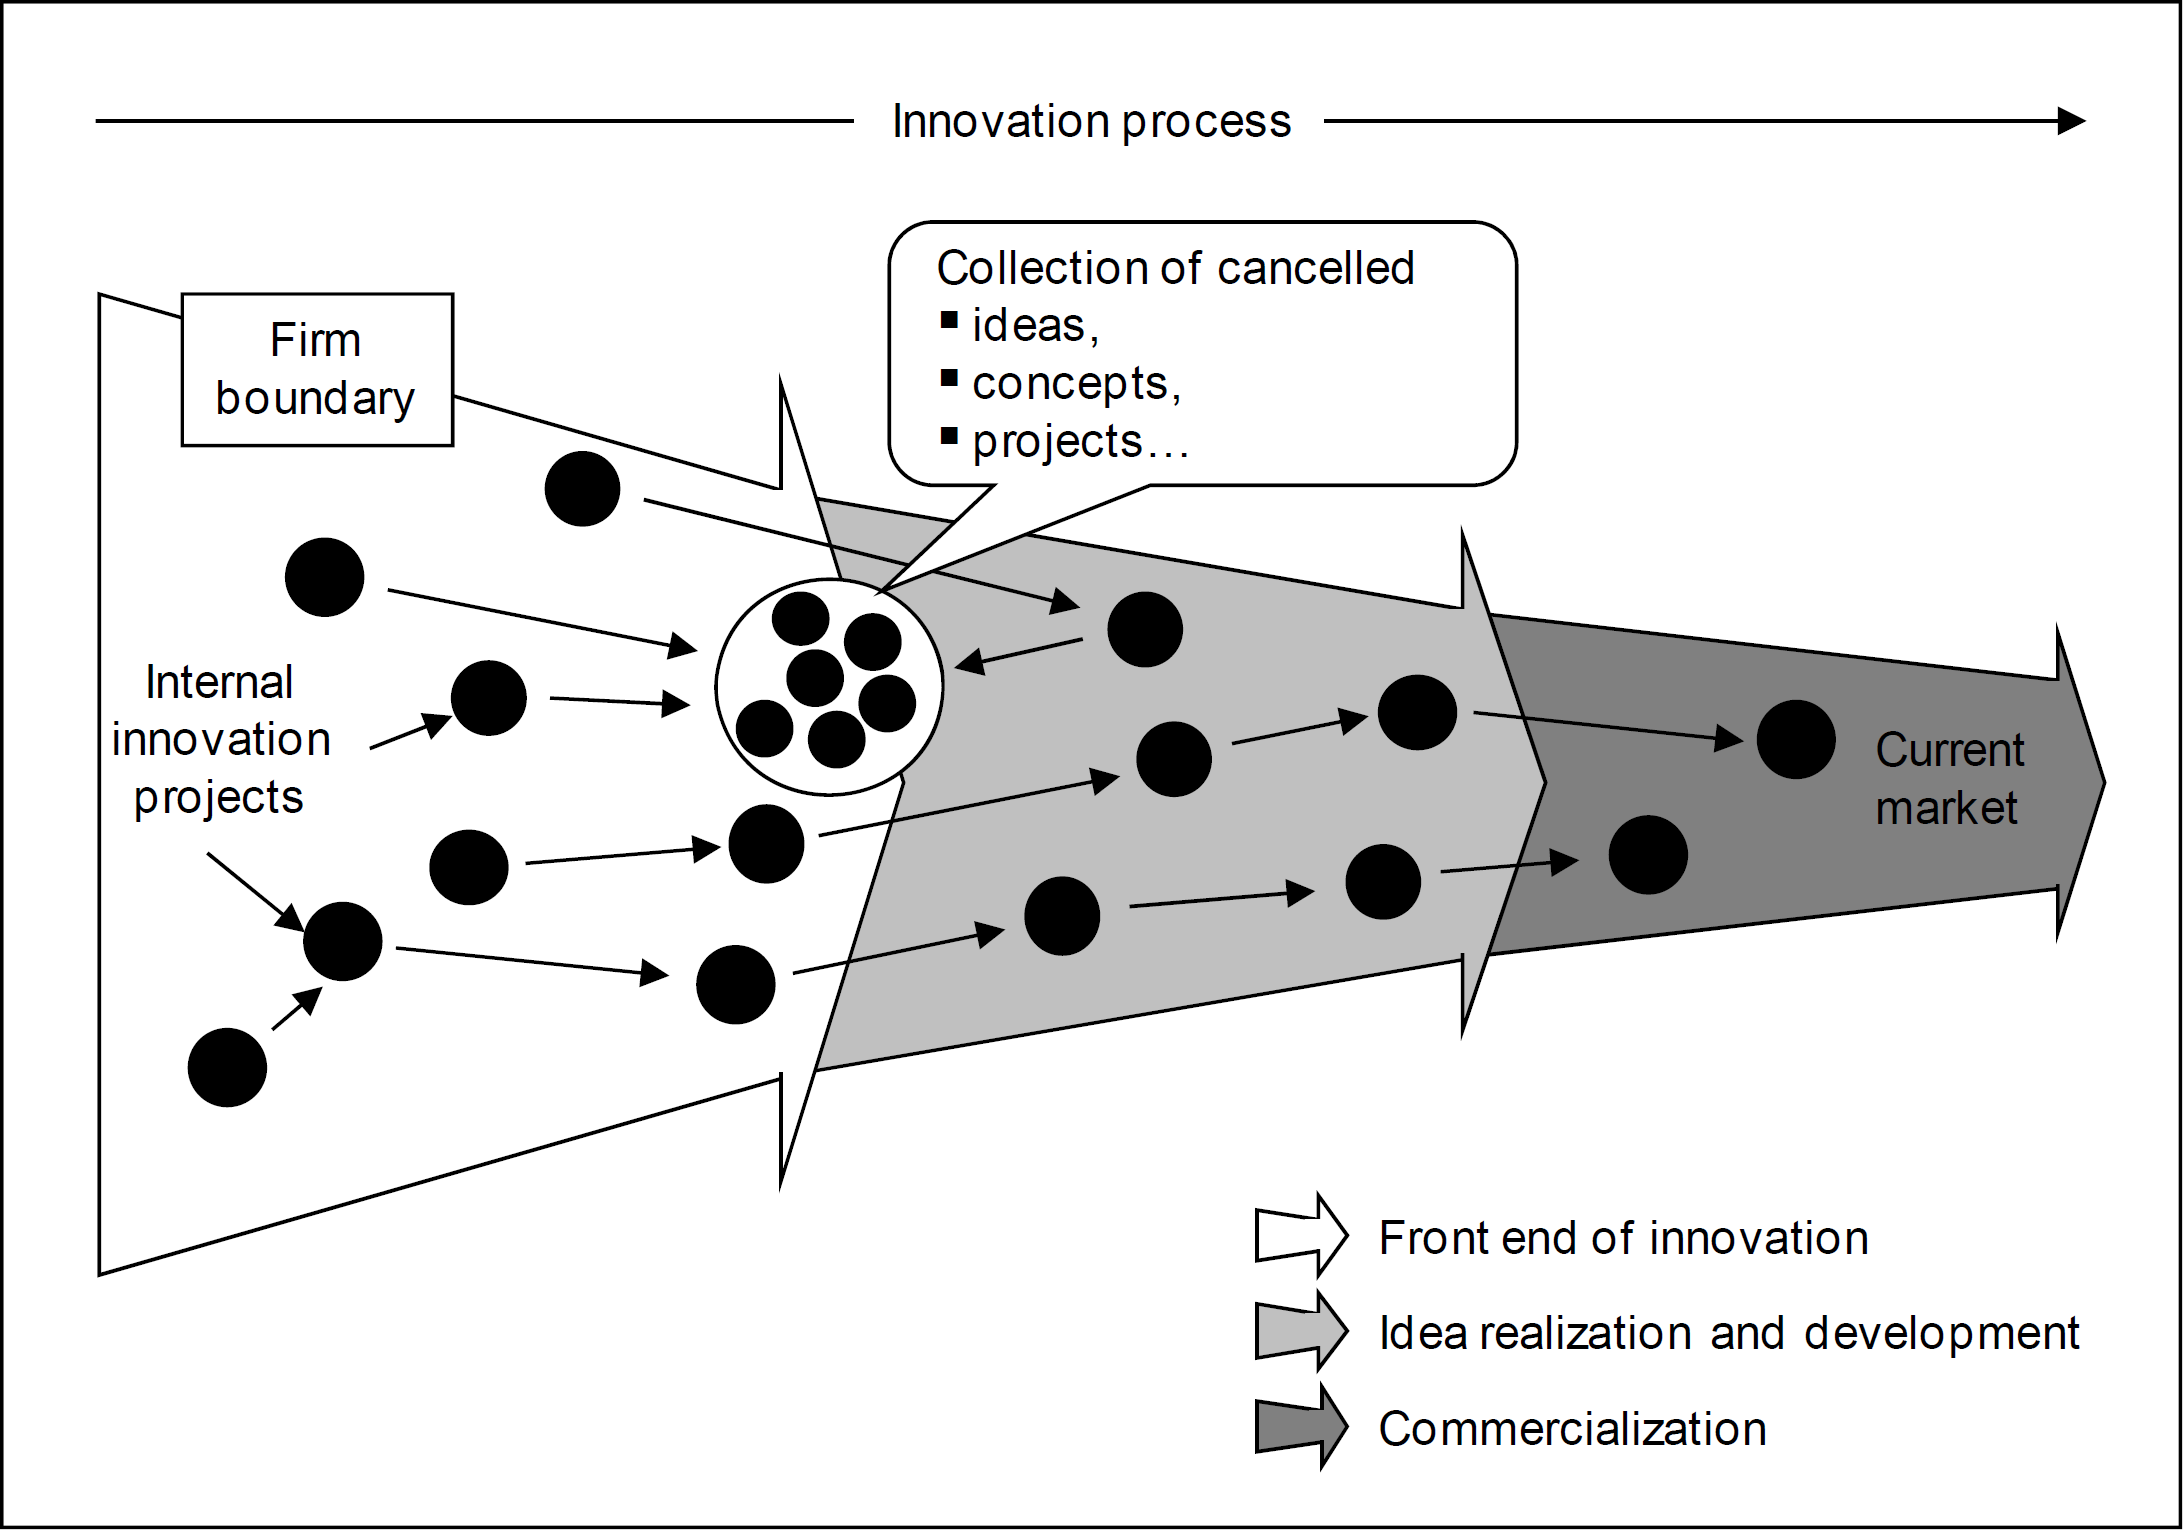
\includegraphics[width=1\textwidth]{ClosedInnovation}
    \caption{Closed Innovation Modell (aus \cite[20]{herzog2011})}
    \label{fig:closedInnovation}
\end{figure}

Nicht alle Ideen können realisiert werden.
Einerseits ist dies ist darauf zurückzuführen, dass Ressourcen in Form von Arbeitskraft oder Wissen nicht ausreichend vorhanden sind.
Andererseits zielt die Idee nicht auf den aktuellen Markt oder es wird vermutet, dass dort keine Akzeptanz herrscht.

Abgelehnte Ideen und abgebrochene Projekte werden beispielsweise in Datenbanken gesammelt.
Von dort werden sie wieder aufgegriffen
oder bleiben ein ungenutzter Teil des geistigen Eigentums eines Unternehmens.



\section{Überblick über Open Innovation}\label{sec:grundlagen-open}

Das Modell der \textit{Open Innovation} ist -- schon rein namentlich -- der Gegensatz der \textit{Closed Innovation}.
Da der Fokus dieser Arbeit auf letzerem liegt,
wird im Folgenden der offene Ansatz lediglich oberflächlich behandelt.
\todo[inline]{... um später besser Vergliechen zu können?}

\begin{figure}[ht!]
    \centering
    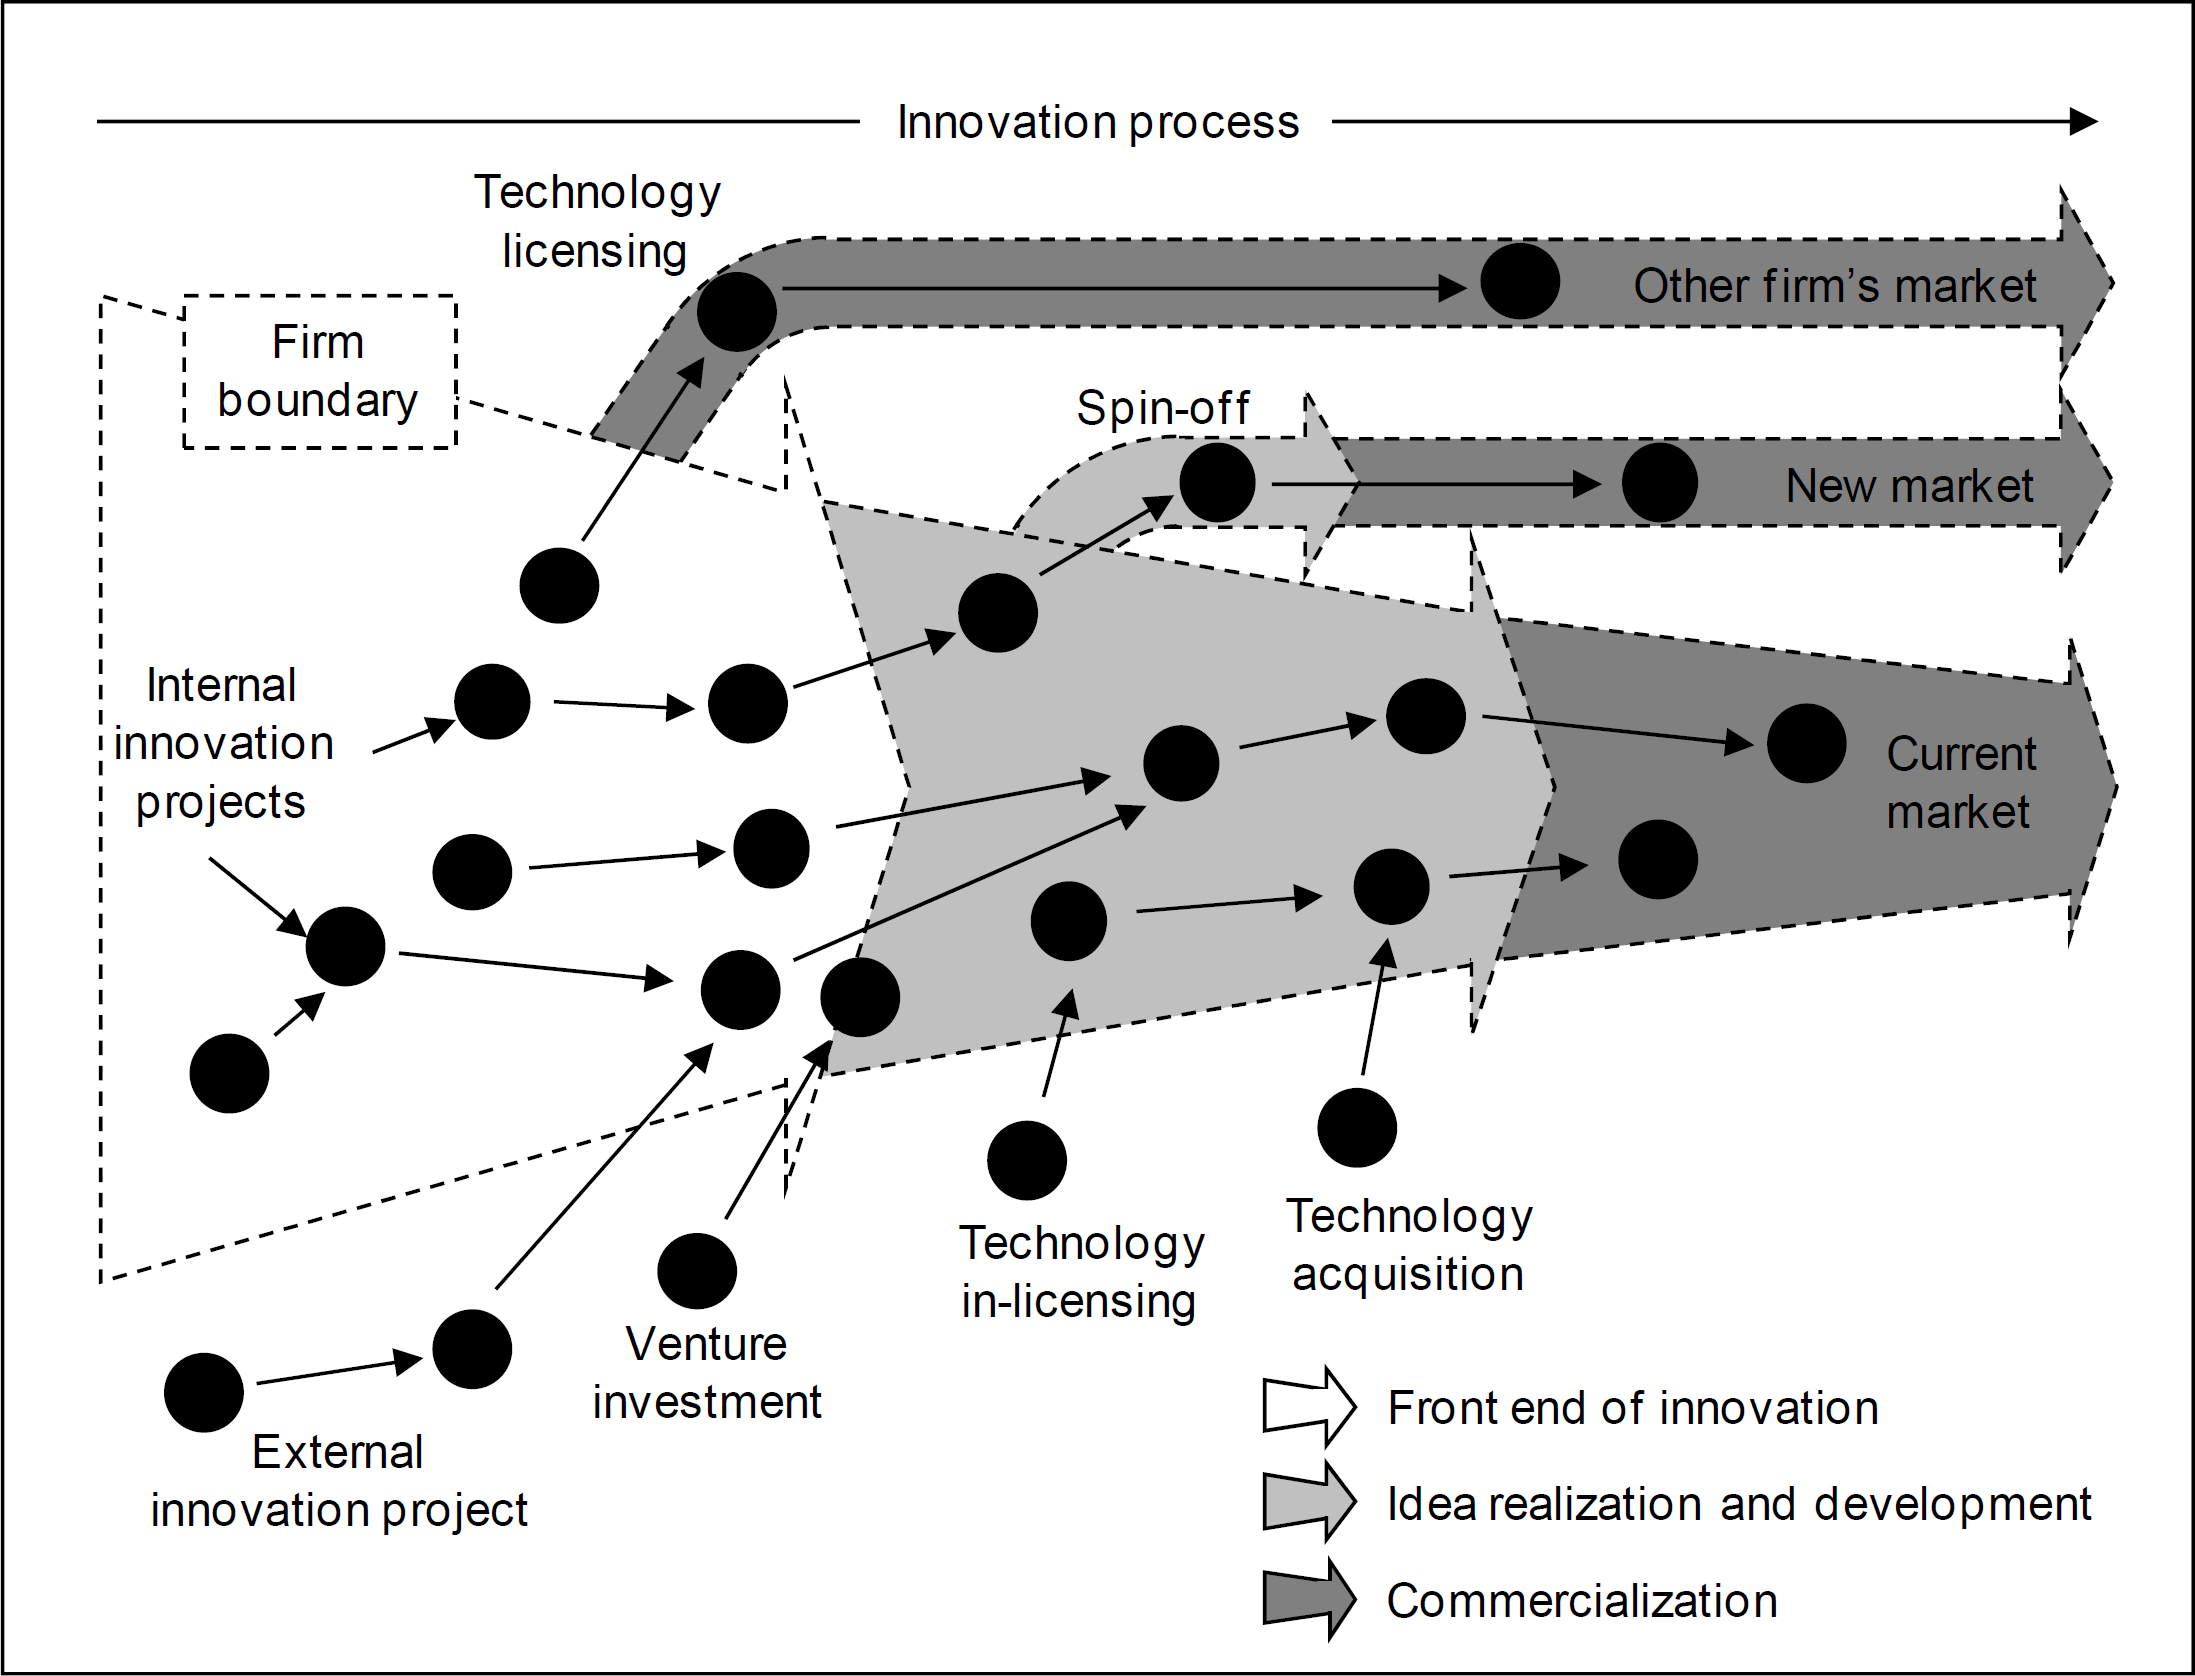
\includegraphics[width=1\textwidth]{OpenInnovation}
    \caption{Open Innovation Modell (aus \cite[23]{herzog2011})}
    \label{fig:openInnovation}
\end{figure}

Wie in \autoref{fig:openInnovation} zu sehen,
sind in der \textit{Open Innovation} die Grenzen eines Unternehmens \enquote{löchrig}.
Dies bedeutet, dass zusätzlich zu den intern entstandenen und entwickelten Innovationen
zusätzlich jederzeit Wissen von außen in den Innovationsprozess einfließt
und Projekte, welche innerhalb des Unternehmens nicht weiter verfolgt werden,
veröffentlicht werden oder genutz werden um neue Märkte zu erschließen.

Details zum \textit{Closed Innovation}-Ansatz können in unter Anderem
in \cite[60\psqq]{chesbrough2003} und \cite[21\psqq]{herzog2011} nachgelesen werden.
\newpage
\section{Bewertung der \textit{Closed Innovation}}\label{sec:bewertung}


\subsection{Vorteile}\label{sec:bewertung-vor}
Ein großer Vorteil der \textit{Closed Innovation} ist die vollständige Kontrolle über den Innovationsprozess.
Das Unternehmen kann die Entwicklung steuern,
um so die eigenen Ziele zu erreichen.
Durch die weitestgehende Unabhängigkeit von Zulieferern besteht auch keine Abhängigkeit zu deren Innovationskraft.

Als Unternehmen, welches sich in einer komfortablen Markposition befindet
und welches die personellen aber vor allem auch finanziellen Ressourcen besitzt,
kann die interne \ac{fe} ausgebaut und gefördert werden.
Auf diesem Weg können viele Ideen generiert und Innovationen entwickelt werden,
was wiederum die Marktmacht stärk oder -- in stark umkämpften Märkten -- zumindest erhält.

Da die entstehenden Innovationen lediglich als selbst vermarktete Produkte veröffentlicht werden,
kann ich ein innovatives Unternehmen Alleinstellungsmerkmale und somit einen Wettbewerbsvorteil gegenüber anderen,
weniger innovativen, Unternehmen sichern.

\subsection{Nachteile}\label{sec:bewertung-nach}
Um im Unternehmen eine erfolgreiche \ac{fe}-Abteilung zu etablieren,
werden hochqualifizierte Fachkräfte benötigt.
Auch die Konkurrenz wirbt um diese Fachkräfte,
wodurch hohe Kosten für die Akquise und das Halten der Mitarbeiter entstehen.

Zusätzlich ist der Erfolg von \textit{Closed Innovation} davon abhängig,
dass die \enquote{besten Fachkräfte} Teil des eigenen Unternehmens sind.
Praktisch ist dies jedoch nicht möglich.

Nach \cite{stevens19973} werden ca. 3000 Ideen benötigt um am Ende ein erfolgreiches Produkt zu erhalten.
Aus diesen Ideen müssen die relevanten ausgewählt und untersucht werden.
Angepasst auf den dreistufigen Innovationsprozess verlassen nur etwa 125 dieser Ideen die erste Stufe
und werden in kleinen Projekten entwickelt.
Im weiteren Verlauf werden von diesen 125 Projekten im Schnitt überschaubare 1,7 Projekte kommerzialisiert.
Es müssen somit viele Ideen gleichzeitig entwickelt werden,
von welchen nur ein geringer Teil später Gewinne einbringt.
Viele der Ideen werden nicht umgesetzt, da deren eigentliches Potential nicht ersichtlich ist.
Insgesamt entstehen somit hohe Kosten und potentielle Gewinne werden nicht erwirtschaftet.

Wie bereits genannt sind Fachkräfte ein großer Faktor für den Erfolg von \textit{Closed Innovation}.
Verlassen diese das Unternehmen, so nehmen sie das gesammelte Wissen mit sich.
Beispielsweise ist es möglich, dass der Mitarbeiter durch einen Konkurrenten abgeworben wird.
Eine andere Ursache für die Fluktuation von Mitarbeitern ist,
dass diese an einem Projekt beteiligt sind,
welches von dem Unternehmen nicht weiterverfolgt werden soll.
Im Gegensatz zum Unternehmen glauben die Mitarbeiter jedoch an den Erfolg ihrer Idee
und entschließen sich diese in einem eigenen oder einem anderen Unternehmen zu realisieren.

Unabhängig von der Art wie der Mitarbeiter das Unternehmen verlässt,
verliert das Unternehmen so einen Teil seines geistigen Eigentums
und kann daraus keine Innovationen und Gewinne mehr generieren.
Schlimmer noch, ein anderes Unternehmen profitiert von den bereits getätigten Investitionen.

In der IT-Branche ist das Wissen auf viele Unternehmen und vor allem zahlreiche Startups verteilt.
Außerdem ist viel Wissen beispielsweise durch Open-Source-Software frei zugänglich.
Wird der Ansatz der \textit{Closed Innovation} streng verfolgt,
so kann auf dieses Wissen jedoch nicht zugegriffen werden.

\subsection{Erwähnenswertes}\label{sec:bewertung-erw}
Vor allem im 20. Jahrhundert ist die \textit{Closed Innovation}
aufgrund der damaligen Wissensumgebung
ein logischer Ansatz um Innovation in einem Unternehmen zu etablieren.

\textit{Closed} und \textit{Open Innovation} sind zwar an sich gegensätzliche Methoden,
sollten aber nicht unbedingt getrennt voneinander betrachtet werden.
Wie in \cite{OpenInno32:online} vorgeschlagen wird,
können die beiden Prinzipen auch kombiniert werden.
Somit kann die interne Innovationskraft stark ausgebaut und geistiges Eigentum aufgebaut werden,
während gleichzeitig die Nachteile der \textit{Closed Innovation} kompensiert werden.

\newpage
\section{Beispiele}\label{sec:beispiele}

\subsection{Verschiedene Unternehmen in der IT-Branche}\label{sec:beispiele-unternehmen}
Chesbrough beschreibt in \cite{chesbrough2003} verschiedene Innovationsansätze von Unternehmen.
Im Folgenden werden die \textit{Closed Innovation}-Ansätze der Unternehmen \textit{Xerox} und \textit{IBM} behandelt.

\paragraph{Xerox \cite[1\psqq]{chesbrough2003}}
Als führendes Unternehmen der amerikanischen Drucker- und Kopiererbranche,
ist ein Xerox Beispiel für die Anwendung von \textit{Closed Innovation}.
1970 gründet das Unternehmen das \ac{parc}.
Dort wurden für die Informationstechnologie wegweisende Technologien wie
Ethernet, graphische Benutzeroberflächen, Textverarbeitungsprogramme und Laserdrucker geboren.

Hierbei ist auffällig, dass - mit Ausnahme der Laserdrucker - keine der Technologien mit Xerox
assoziiert werden.
Dem Unternehmen ist es nicht gelungen einen Nutzen aus diesen Innovationen zu ziehen.

Durch Übernahme von Mitarbeiter gelangt beispielsweise das Wissen zu graphischen Benutzeroberflächen bei Apple
und das Textverarbeitungsprogramm wird bei Microsoft zu dem heute weit verbreiteten \textit{Microsoft Word}.

Ethernet hingegen verlässt das Unternehmen durch dessen Erfinder Robert Metcalfe,
da er nicht warten wollte bis Xerox diese Technologie kommerzialisiert \cite[81]{chesbrough2003}.
Auf ähnliche Weiße ensteht das bekannte Unternehmen \textit{Adobe}.



\paragraph{IBM \cite[93\psqq]{chesbrough2003}}
Mit der Gründung eines Forschungszentrum im Jahre 1945 verfolgt das Technologieunternehmen ebenfalls den \textit{Closed Innovation}-Ansatz.
Zu den Innovationen IBMs zählen beispielsweise
\textit{RAMAC 305} -- die erste Festplatte,
\textit{FORTRAN} -- die erste höhere Programmiersprache und
Magnetbänder.

1964 definiert IBM durch das \textit{System 360} den damaligen Standard für Mainframe-Computer (Großrechner).
Für \textit{Closed Innovation} typisch entwickelt IBM nicht nur das System an sich,
sondern unter anderem auch Schlüsselkomponenten, das Betriebssystem, Software und sogar die Tastatur und die Stromversorgung.
IBM war zu diesen Entwicklungen, da das gesamte System auf einer komplett neuen Architektur basiert.
Um auf Zulieferer zurückzugreifen müsste diese zuvor kosten- und zeitintensiv geschult werden.

Im Vergleich zu Xerox ist IBM mit diesem Ansatz deutlich erfolgreicher.
Ab 1980 wird dieser Erfolg jedoch gebremst.
Durch die geänderte Wissenslandschaft im Bereich der Informatik haben auch andere Unternehmen
Zugriff auf notwendiges Wissen und können ihre Ideen vermarkten.
IBM vierliert so seine Alleinstellung als \enquote{Ideenmaschine}
und beginnt die Transformation von der \textit{Closed} zur \textit{Open Innovation}.


\subsection{SAP}\label{sec:beispiele-sap}
Im Jahr 1972 gründen Claus Wellenreuther, Hans-Werner Hector, Klaus Tschira, Dietmar Hopp und Hasso Plattner das Unternehmen.
Ziel der fünf ehemaligen IBM Mitarbeiter war es
Standardsoftware zur Echtzeit-\linebreak Verarbeitung von Daten für andere Unternehmen zu entwickeln.

Diese Entwicklung sollte eigentlich innerhalb von IBM geschehen.
Jedoch gestatte das Unternehmen dies nicht und wollte die Entwicklung durch andere Mitarbeiter durchführen lassen.
Daraufhin entschlossen sich die fünf SAP-Gründer ihre Idee in einem eigenen Unternehmen umzusetzen. \cite{SAPCompa72:online}

\paragraph{Gesamtes Unternehmen}\label{sec:beispiele-sap-gesamt}
Das Unternehmen SAP als solches pflegt eine überwiegend offene Unternehmenskultur.
Es ist bekannt dafür durch zahlreiche Akquisitionen das unternehmensinterne geistige Eigentum zu erweitern.

Durch die Veröffentlichung von Open-Source-Software sind zahlreiche Bibliotheken wie \textit{OpenUI5} offen verfügbar.

Auch \enquote{klassische} SAP-Anwendungen sind auf Offentheit ausgelegt.
Durch entsprechende Schnittstellen und Tools wird es sogenannten \enquote{Partnern}
ermöglicht das vorhandene Programm zu erweitern.

Das Unternehmen pflegt zudem eine intensive Kooperation mit anderen Unternehmen
wie Apple \cite{Appleund81:online} und Microsoft \cite{Microsof58:online}.
Kunden werden mit Hilfe von \textit{Design Thinking} \cite{SAPDesig64:online} früh in den Entwicklungsprozess eingebunden.



\paragraph{\ac{sac}}\label{sec:beispiele-sap-sac}
Hinter diesen Begriff steckt eine Analyse- und Planungssoftware des Unternehmens SAP.
Als \enquote{Cloudsoftware} wird die Anwendung auf SAP-eigenen Servern zur Verfügung gestellt.
Auch die regelmäßige Aktualisierung der Software gehört zu den Aufgaben der SAP.

Im Fall von \ac{sac} wird dies alle zwei Wochen durchgeführt.
Diese kurzen Entwicklungs- und damit Feedback-Zyklen führen zu einem regen Austausch zwischen der Entwicklungsabteilung und den Kunden.
Mit ausgewählten Kunden wird diese Kooperation noch weiter intensiviert.

Ein weiterer Indikator für die Offentheit der Entwicklung sind die verwendeten Technologien.
Grundlegend basiert die Anwendung zwar auf SAP-eigenen Technologien,
aber es werden auch am Markt etablierte Bibliotheken wie \textit{React} und andere quelloffene Bausteine verwendet.

\newpage
\section{Fazit}\label{sec:fazit}
Wie in Kapitel \ref{sec:bewertung} gezeigt, überwiegen bei der \textit{Closed Innovation}
die Nachteile klar die Vorteile.
Aufgrund der seinerzeit vorherrschenden Wissenslandschaft und des damaligen Arbeitsmarkts
hatte dieses Paradigma vor allem im 20. Jahrhundert seine Berechtigung.

Doch mittlerweile hat sich dies geändert.
Universitäten sind offener gegenüber praxisorientierter Forschung.
Qualifizierte Arbeitskräfte sind einfacher verfügbar.
Zusätzlich hat die Komplexität der Innovationen so weit zugenommen,
dass das benötigte Wissen durch ein einzelnes Unternehmen nicht mehr erfasst werden kann.

Somit ist \textit{Closed Innovation} vor allem in der IT-Industrie als nicht mehr zeitgemäß anzusehen.
\newpage

%\printacronyms{}
\printbibliography{}
\end{document}
